\documentclass[10pt]{article}
\usepackage[paperwidth=39cm, paperheight=39cm, margin=1cm]{geometry}
% Usuń numerację stron.
\pagestyle{empty}

\usepackage{tikz}
% Import do ustalania końcówek strzałek.
\usetikzlibrary{arrows.meta}

% Zmniejsz interlinię.
\linespread{0.9}

% Importy do białych konturów napisów.
\usepackage[T1]{fontenc}
\usepackage{pslatex}
\usepackage{contour}
\usepackage{color}
\contourlength{1pt} % Grubość konturu
\contournumber{50}  % Liczba powtórzeń

% Ustaw czcionkę bezszeryfową.
\renewcommand{\familydefault}{\sfdefault}

\begin{document}
\begin{figure}[p]
\centering
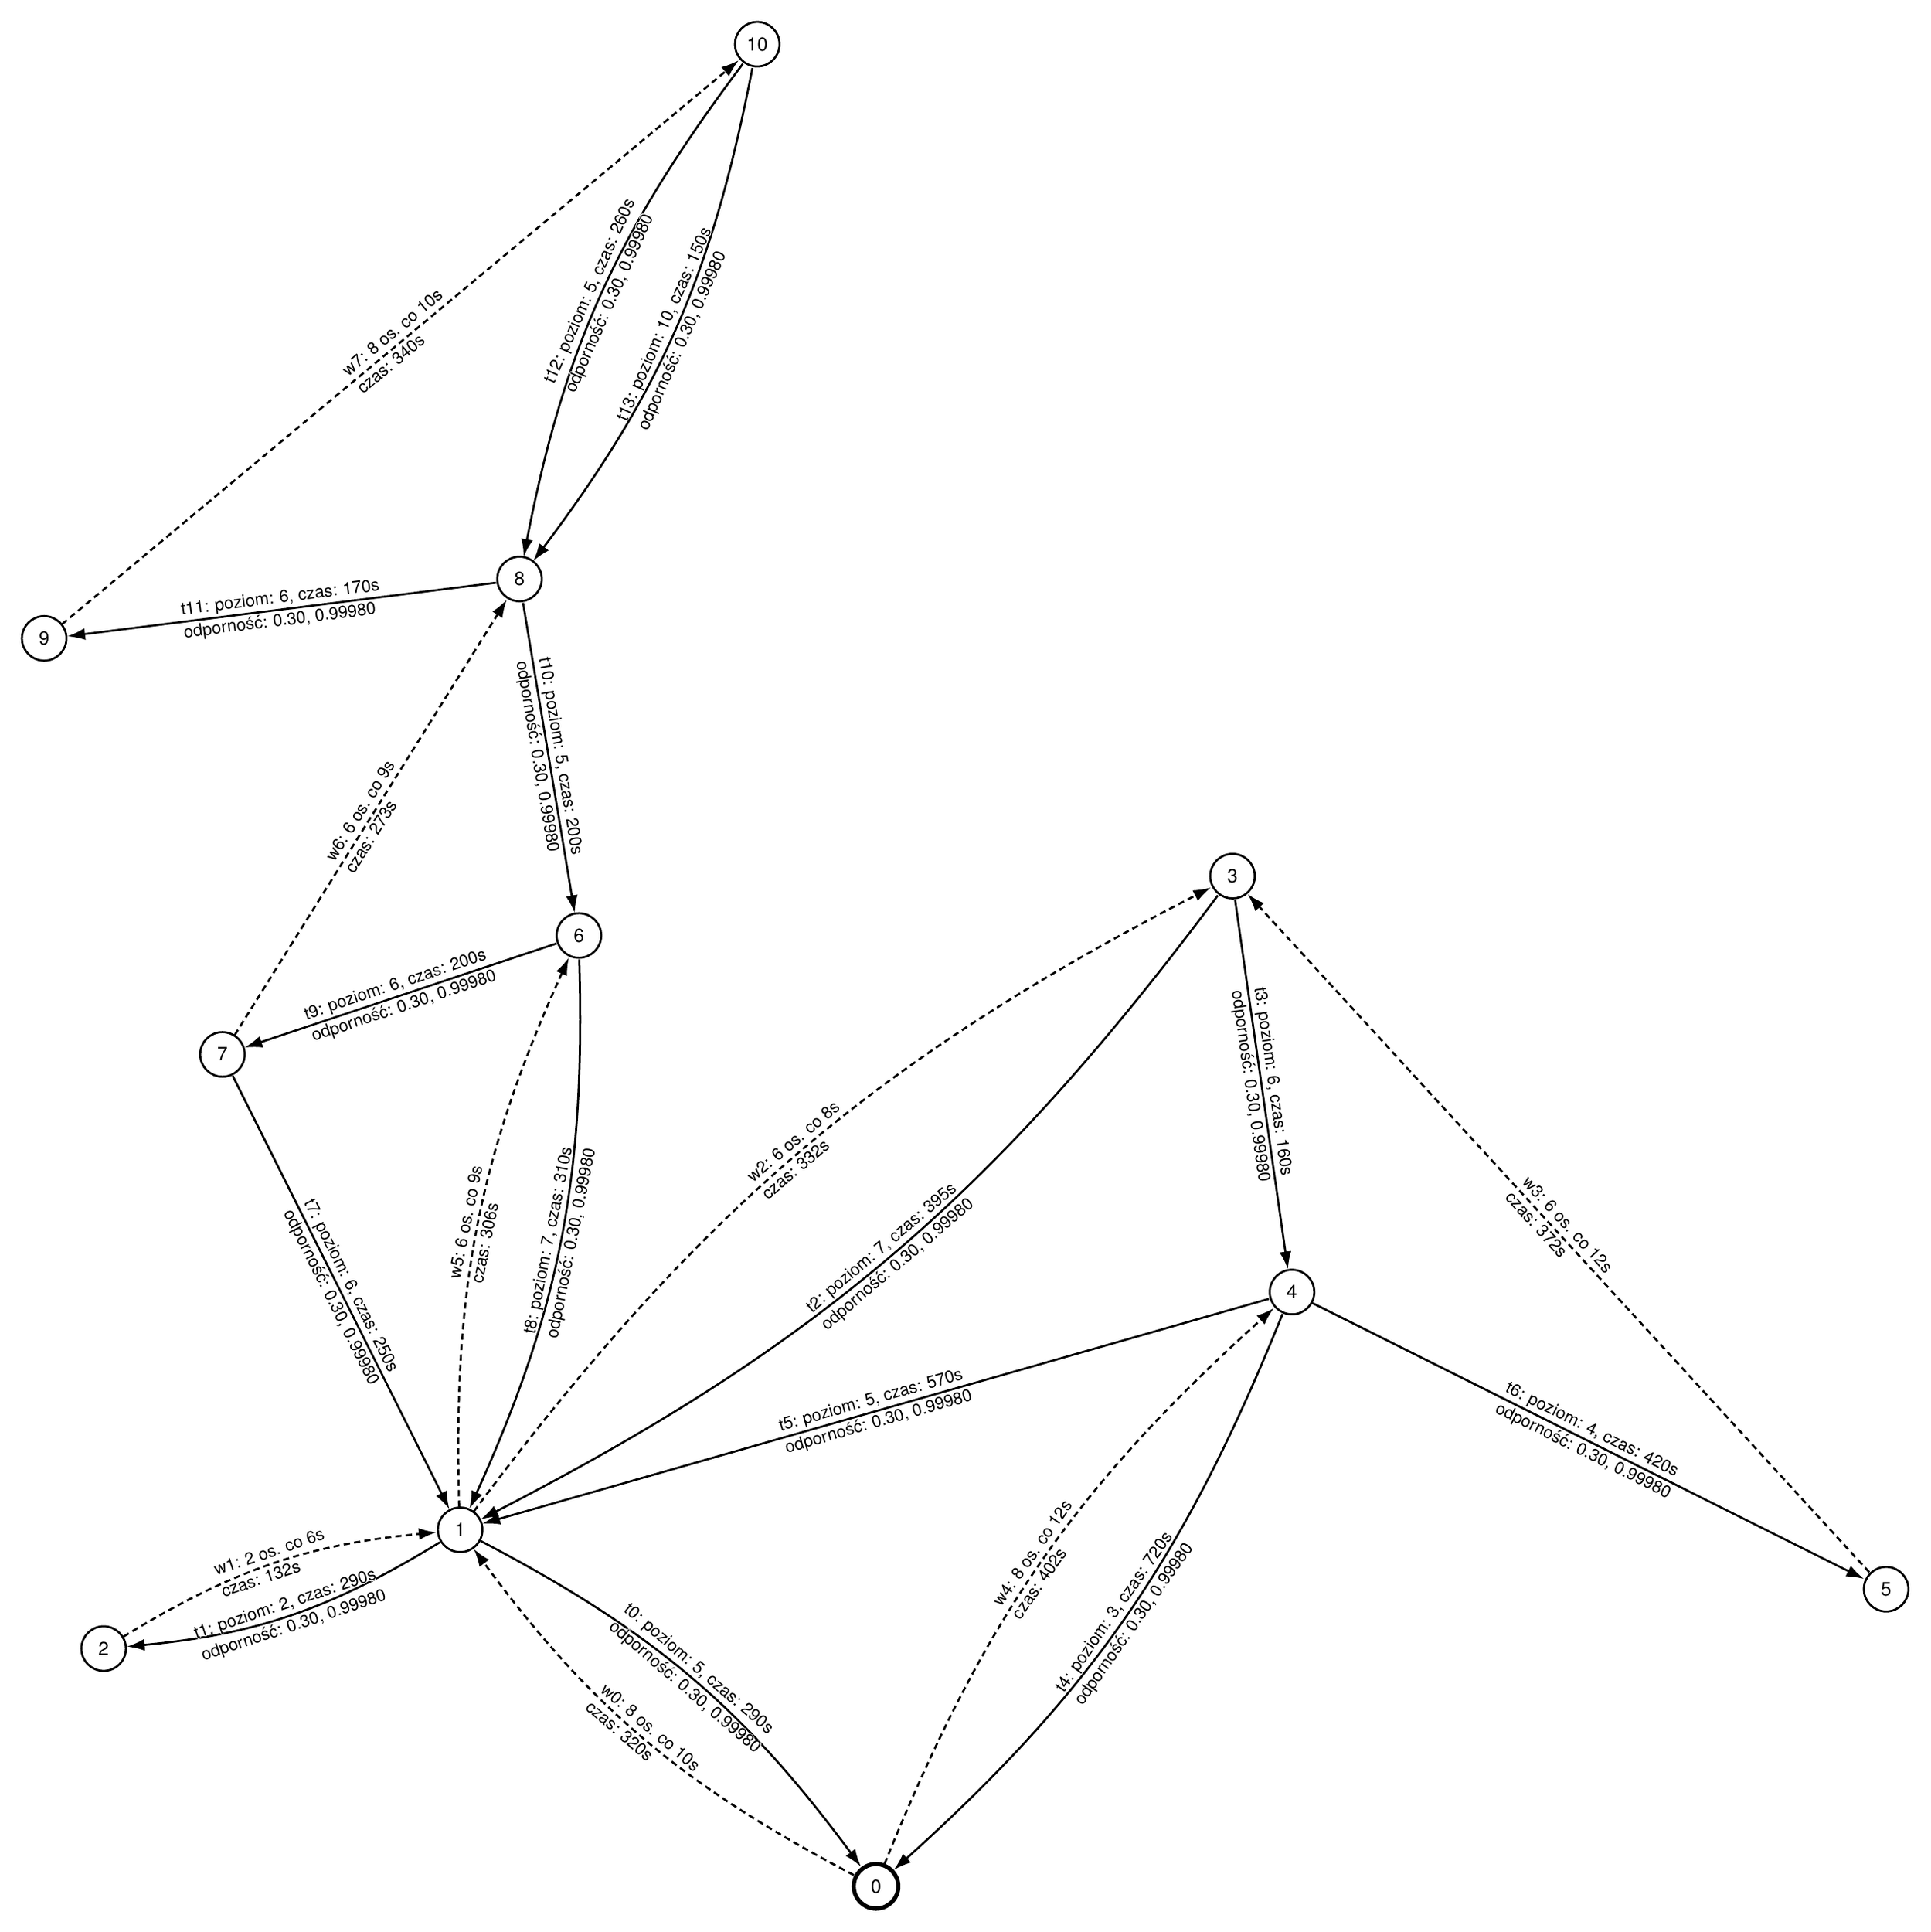
\begin{tikzpicture}[scale=100]
    \tikzset{
        % Style węzłów i krawędzi.
        wezel grafu/.style={circle,draw,minimum size=0.75cm,inner sep=0,line width=0.35mm},
        krawedz grafu/.style={-{Latex[length=3mm, width=2mm]},sloped,centered,line width=0.35mm,font=\small}
    }
    % Węzły:
    \node[wezel grafu,line width=0.7mm] (0) at (16/100, 2/100) {0};
    \node[wezel grafu] (1) at (9/100, 8/100) {1};
    \node[wezel grafu] (2) at (3/100, 6/100) {2};
    \node[wezel grafu] (3) at (22/100, 19/100) {3};
    \node[wezel grafu] (4) at (23/100, 12/100) {4};
    \node[wezel grafu] (5) at (33/100, 7/100) {5};
    \node[wezel grafu] (6) at (11/100, 18/100) {6};
    \node[wezel grafu] (7) at (5/100, 16/100) {7};
    \node[wezel grafu] (8) at (10/100, 24/100) {8};
    \node[wezel grafu] (9) at (2/100, 23/100) {9};
    \node[wezel grafu] (10) at (14/100, 33/100) {10};
    % Krawedzie:
    \path[draw]
    (0) edge[krawedz grafu, bend left=13, densely dashed] node {
        \begin{tabular}{l}
            \contour{white}{w0: 8 os. co 10s} \\
            \contour{white}{czas: 320s}
        \end{tabular}
    } (1)
    (1) edge[krawedz grafu, bend left=13] node {
        \begin{tabular}{l}
            \contour{white}{t0: poziom: 5, czas: 290s} \\
            \contour{white}{odporność: 0.30, 0.99980}
        \end{tabular}
    } (0)
    (0) edge[krawedz grafu, bend left=13, densely dashed] node {
        \begin{tabular}{l}
            \contour{white}{w4: 8 os. co 12s} \\
            \contour{white}{czas: 402s}
        \end{tabular}
    } (4)
    (4) edge[krawedz grafu, bend left=13] node {
        \begin{tabular}{l}
            \contour{white}{t4: poziom: 3, czas: 720s} \\
            \contour{white}{odporność: 0.30, 0.99980}
        \end{tabular}
    } (0)
    (1) edge[krawedz grafu, bend left=13] node {
        \begin{tabular}{l}
            \contour{white}{t1: poziom: 2, czas: 290s} \\
            \contour{white}{odporność: 0.30, 0.99980}
        \end{tabular}
    } (2)
    (2) edge[krawedz grafu, bend left=13, densely dashed] node {
        \begin{tabular}{l}
            \contour{white}{w1: 2 os. co 6s} \\
            \contour{white}{czas: 132s}
        \end{tabular}
    } (1)
    (1) edge[krawedz grafu, bend left=13, densely dashed] node {
        \begin{tabular}{l}
            \contour{white}{w2: 6 os. co 8s} \\
            \contour{white}{czas: 332s}
        \end{tabular}
    } (3)
    (3) edge[krawedz grafu, bend left=13] node {
        \begin{tabular}{l}
            \contour{white}{t2: poziom: 7, czas: 395s} \\
            \contour{white}{odporność: 0.30, 0.99980}
        \end{tabular}
    } (1)
    (4) edge[krawedz grafu] node {
        \begin{tabular}{l}
            \contour{white}{t5: poziom: 5, czas: 570s} \\
            \contour{white}{odporność: 0.30, 0.99980}
        \end{tabular}
    } (1)
    (1) edge[krawedz grafu, bend left=13, densely dashed] node {
        \begin{tabular}{l}
            \contour{white}{w5: 6 os. co 9s} \\
            \contour{white}{czas: 306s}
        \end{tabular}
    } (6)
    (6) edge[krawedz grafu, bend left=13] node {
        \begin{tabular}{l}
            \contour{white}{t8: poziom: 7, czas: 310s} \\
            \contour{white}{odporność: 0.30, 0.99980}
        \end{tabular}
    } (1)
    (7) edge[krawedz grafu] node {
        \begin{tabular}{l}
            \contour{white}{t7: poziom: 6, czas: 250s} \\
            \contour{white}{odporność: 0.30, 0.99980}
        \end{tabular}
    } (1)
    (3) edge[krawedz grafu] node {
        \begin{tabular}{l}
            \contour{white}{t3: poziom: 6, czas: 160s} \\
            \contour{white}{odporność: 0.30, 0.99980}
        \end{tabular}
    } (4)
    (5) edge[krawedz grafu, densely dashed] node {
        \begin{tabular}{l}
            \contour{white}{w3: 6 os. co 12s} \\
            \contour{white}{czas: 372s}
        \end{tabular}
    } (3)
    (4) edge[krawedz grafu] node {
        \begin{tabular}{l}
            \contour{white}{t6: poziom: 4, czas: 420s} \\
            \contour{white}{odporność: 0.30, 0.99980}
        \end{tabular}
    } (5)
    (6) edge[krawedz grafu] node {
        \begin{tabular}{l}
            \contour{white}{t9: poziom: 6, czas: 200s} \\
            \contour{white}{odporność: 0.30, 0.99980}
        \end{tabular}
    } (7)
    (8) edge[krawedz grafu] node {
        \begin{tabular}{l}
            \contour{white}{t10: poziom: 5, czas: 200s} \\
            \contour{white}{odporność: 0.30, 0.99980}
        \end{tabular}
    } (6)
    (7) edge[krawedz grafu, densely dashed] node {
        \begin{tabular}{l}
            \contour{white}{w6: 6 os. co 9s} \\
            \contour{white}{czas: 273s}
        \end{tabular}
    } (8)
    (8) edge[krawedz grafu] node {
        \begin{tabular}{l}
            \contour{white}{t11: poziom: 6, czas: 170s} \\
            \contour{white}{odporność: 0.30, 0.99980}
        \end{tabular}
    } (9)
    (10) edge[krawedz grafu, bend left=-13] node {
        \begin{tabular}{l}
            \contour{white}{t12: poziom: 5, czas: 260s} \\
            \contour{white}{odporność: 0.30, 0.99980}
        \end{tabular}
    } (8)
    (10) edge[krawedz grafu, bend left=13] node {
        \begin{tabular}{l}
            \contour{white}{t13: poziom: 10, czas: 150s} \\
            \contour{white}{odporność: 0.30, 0.99980}
        \end{tabular}
    } (8)
    (9) edge[krawedz grafu, densely dashed] node {
        \begin{tabular}{l}
            \contour{white}{w7: 8 os. co 10s} \\
            \contour{white}{czas: 340s}
        \end{tabular}
    } (10)
    ;
\end{tikzpicture}

\end{figure}
\end{document}
